\documentclass{assignment}

\usepackage{fancyvrb}
\usepackage{url}

\mytitle{C4M: Medical Document Retrieval Worksheet}

\begin{document}

Sample documents:

\begin{center}
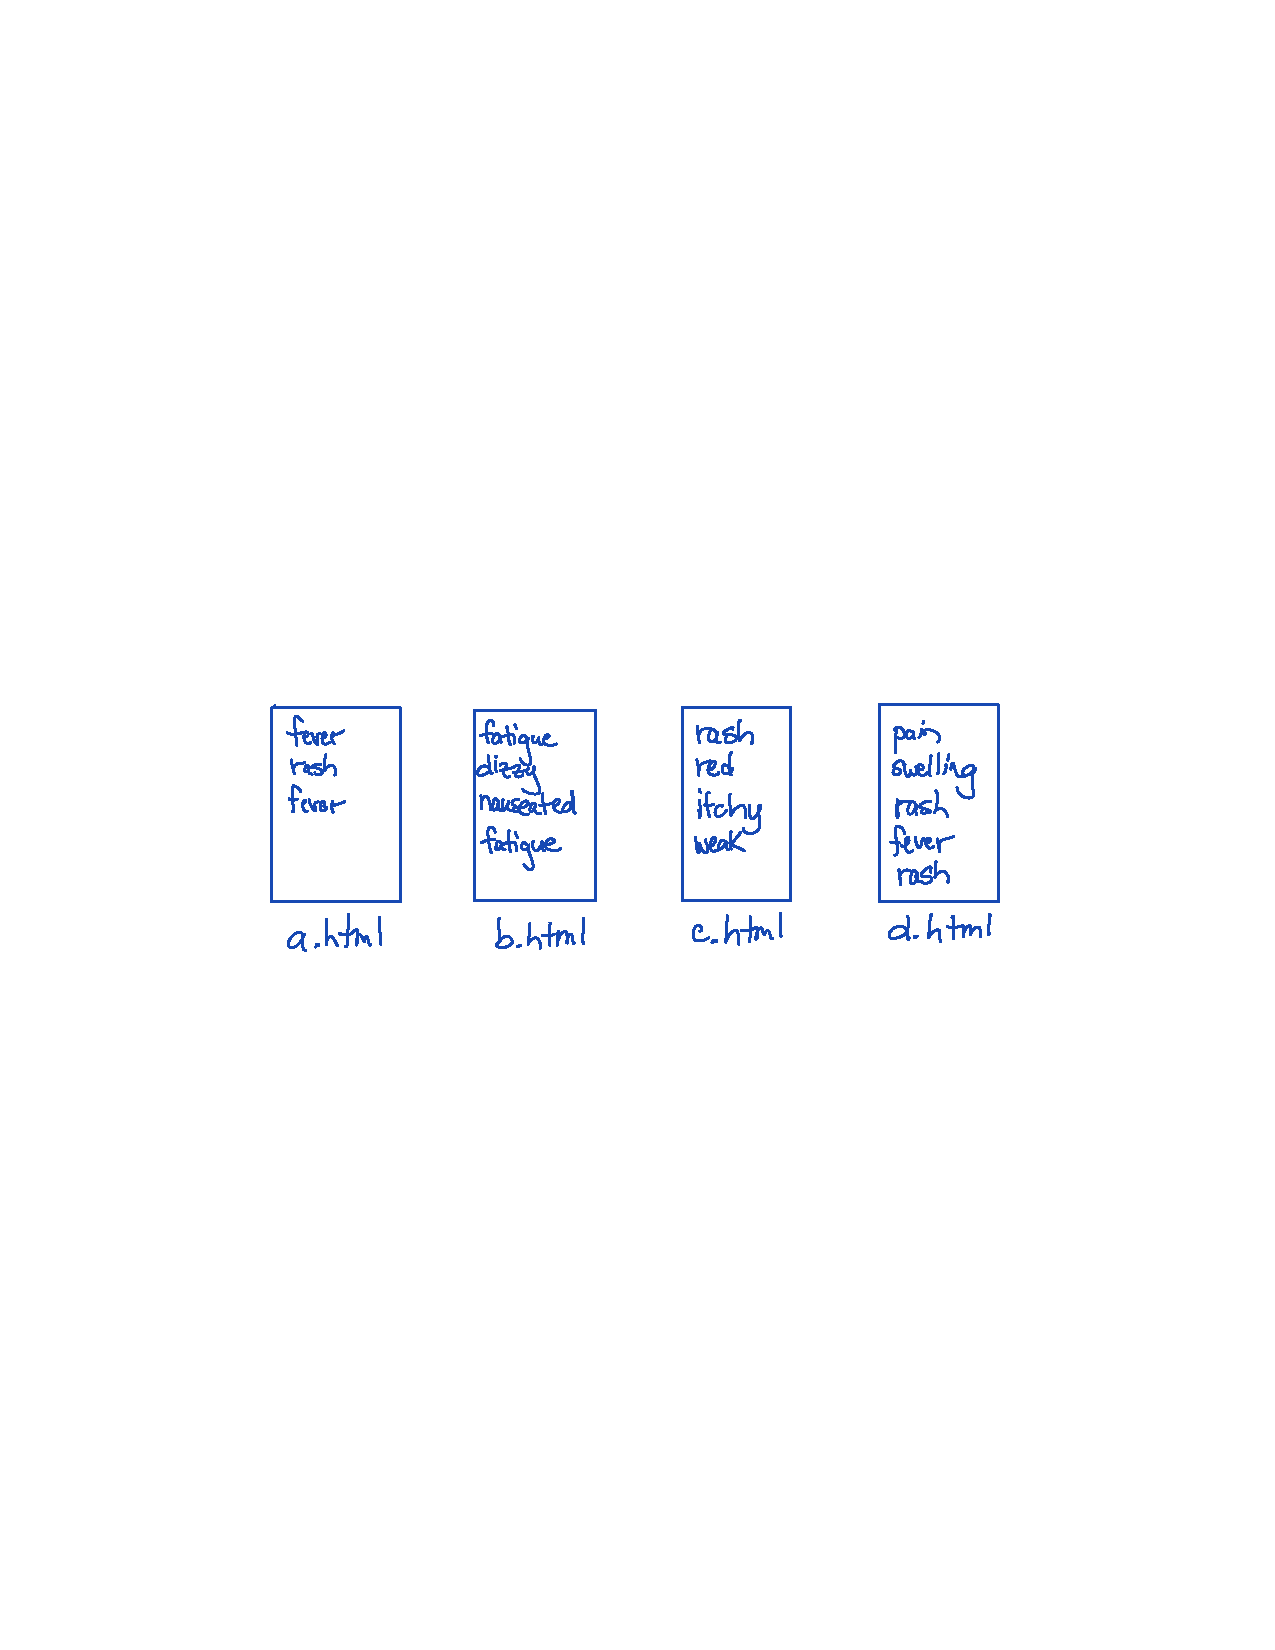
\includegraphics[width=6in]{sample_documents.pdf}
\end{center}
\vspace*{-0.5cm}
Term frequency / inverse document frequency:

\hspace*{0.5 in}$TF(k, d) =
  \begin{cases}
    0       & \text{if } k \text{ does not appear in } d \\
    1       & \text{otherwise}
    \\
    \end{cases}$

\hspace*{0.5 in}$\text{IDF}(k, D) =
     \log \frac{ \quad \text{ No. of docs in } D }{ \quad \text{ No. of docs in } D \text{ that contain } k} $

\hspace*{0.5 in}$\text{TF-IDF}(k, d, D) = TF(t, d) * IDF(k, D)$

$k$ represents a keyword, $d$ represents a document, and $D$ represents the set of all documents.

\begin{enumerate}

\item Query: nauseated
\begin{enumerate}
\item $\text{IDF}(k, D) = $\\

\item Complete the \code{doc\_to\_score} dictionary, where each key represents a document and each value represents that document's $\text{TF-IDF}$ score.
\begin{verbatim}
doc_to_score = {'a':            ,
                'b':            ,
                'c':            ,
                'd':             }
\end{verbatim}
\item Best match:
\end{enumerate}

\item Query: fever rash
\begin{enumerate}
\item $\text{IDF}(k_1, D) = $\\

$\text{IDF}(k_2, D) = $\\


\item Complete the \code{doc\_to\_score} dictionary, where each key represents a document and each value represents that document's $\text{TF-IDF}$ score.
\begin{verbatim}
doc_to_score = {'a':            ,
                'b':            ,
                'c':            ,
                'd':             }
\end{verbatim}
\item Best match:

\end{enumerate}

\end{enumerate}
\end{document}
